\chapter{Interfaz de datos de entrada y salida}
% ----------------------

\label{C:Interfaz de datos de entrada y salida}

\section{Diagrama de bloques de la interfaz de datos}
Para la adquisición de las variables a controlar y el ingreso de datos de configuración por un lado, y para la visualización de variables y manejo del actuador de potencia, se propone el diagrama de bloques de la figura~\ref{F:diagrama_digital}. Se pretende controlar la tensión y corriente de salida en base al algoritmo de control del capitulo anterior que esta vinculado directamente con el ajuste de las referencias impuestas con un teclado numérico. A su vez, por el bus I2C se lleva a cabo la lectura de la tensión y corriente de salida mediante un convertidor AD de alta resolución de 16 bits mientras que los datos procesados se despliegan en un display OLED o LCD. En el display se visualiza la tensión y corriente de salida medidas, la tensión y corriente configurada deseada, y el modo de operación del sistema (CV o CI) así como también si la carga se encuentra conectada o desconectada entre otras funciones. Se agrega además, un comando de acople y desacople de la carga mediante e accionamiento de un relé.

\begin{figure} [H]
    \centering
    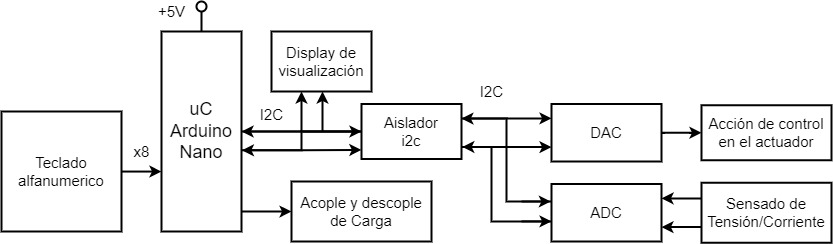
\includegraphics[scale=0.5]{./imagenes/diagrama_digital.jpg}
    \caption{Diagrama de bloques de la interfaz de datos.}
    \label{F:diagrama_digital}
\end{figure}

\section{Componentes de la etapa digital.}
Esta sección del informe está dedicada a desglosar y describir en detalle los componentes esenciales que constituyen la interfaz de manejo de datos de una fuente CC. La comprensión de cada componente, su función y su interacción con otros elementos es fundamental para diseñar un sistema confiable.\par 
Los componentes que se abordarán incluyen microcontroladores, convertidores analógico-digital (ADC), convertidores digital-analógico (DAC), sensores de corriente y voltaje, así como los circuitos de comunicación y control. Cada uno de estos elementos desempeña un rol específico y crítico en la gestión y monitoreo del suministro de energía. A través de esta sección, se explicarán las características técnicas de estos componentes, su importancia en el contexto del diseño de la fuente DC y cómo se integran para formar una unidad cohesiva y funcional.

\subsection{Microcontrolador Arduino Nano.}
El Arduino Nano es un microcontrolador compacto y versátil ampliamente reconocido por su facilidad de uso y sus diversas capacidades. Diseñado por Arduino LLC, este dispositivo ofrece un rendimiento sólido en un formato pequeño, lo que lo convierte en una opción popular para una amplia gama de aplicaciones en el ámbito de la electrónica amateur y profesional.\par 
Con su arquitectura avanzada y un conjunto completo de características, el Arduino Nano es ideal para proyectos que requieren control preciso y eficiente, así como para la interacción con diversos sensores y actuadores. Su capacidad para manejar operaciones en tiempo real lo hace adecuado para aplicaciones que van desde sistemas de automatización del hogar hasta dispositivos portátiles y gadgets interactivos.

\underline{Programación}: \par 
La programación del Arduino Nano se realiza utilizando el entorno de desarrollo integrado (IDE) de Arduino, que proporciona una interfaz intuitiva para escribir, cargar y depurar código. Compatible con una amplia variedad de bibliotecas y herramientas, el IDE de Arduino simplifica el proceso de desarrollo, permitiendo a los usuarios concentrarse en la lógica de su proyecto sin preocuparse por los detalles de bajo nivel del hardware.

\subsection{Teclado de membrana 4x4.}
El teclado de membrana matricial 4x4 autoadhesivo es un dispositivo de entrada que se utiliza comúnmente en aplicaciones electrónicas donde se requiere una interfaz de usuario simple y compacta. Consiste en una delgada lámina de material flexible que contiene una matriz de botones dispuestos en filas y columnas, con un total de 16 botones en este caso particular como se observa en la Figura \ref{F:teclado4x4} (4 filas x 4 columnas). \par 
Cada botón en el teclado de membrana está interconectado mediante una disposición de líneas conductoras en la membrana. Estas líneas están organizadas de manera que forman una matriz, permitiendo la detección de la ubicación específica de la tecla presionada. El funcionamiento del teclado de membrana matricial implica un proceso de escaneo continuo de todas las filas y columnas para detectar la presencia de un botón presionado. Cuando un botón se presiona, se cierra un circuito entre la fila y la columna correspondientes, lo que indica al microcontrolador la ubicación de la tecla activada.

\begin{figure}[H]
    \centering 
    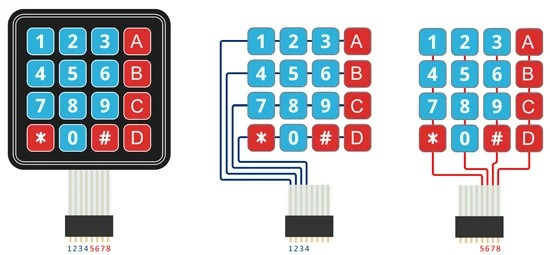
\includegraphics[scale=0.5]{./imagenes/Teclado Matricial 4x4_2.jpg}
    \caption{Ilustración del teclado de membrana, indicando sus filas y columnas.}
    \label{F:teclado4x4}
\end{figure}

\subsection{Display OLED SSD1306.}
El display OLED SSD1306 elegido para el proyecto utiliza comunicación I2C y ofrece una resolución de 128x64 píxeles. En la Figura \ref{F:display} se presenta una imagen del display, que opera dentro de un rango de voltaje de 3.3 a 5.5 V, lo cual lo hace compatible con el microcontrolador seleccionado. En esta pantalla se mostrará tanto el menú de funcionamiento, los modos de operación además de un indicador a tiempo real de las magnitudes registradas. Será el vínculo principal entre el usuario y la fuente.

\begin{figure}[H]
    \centering 
    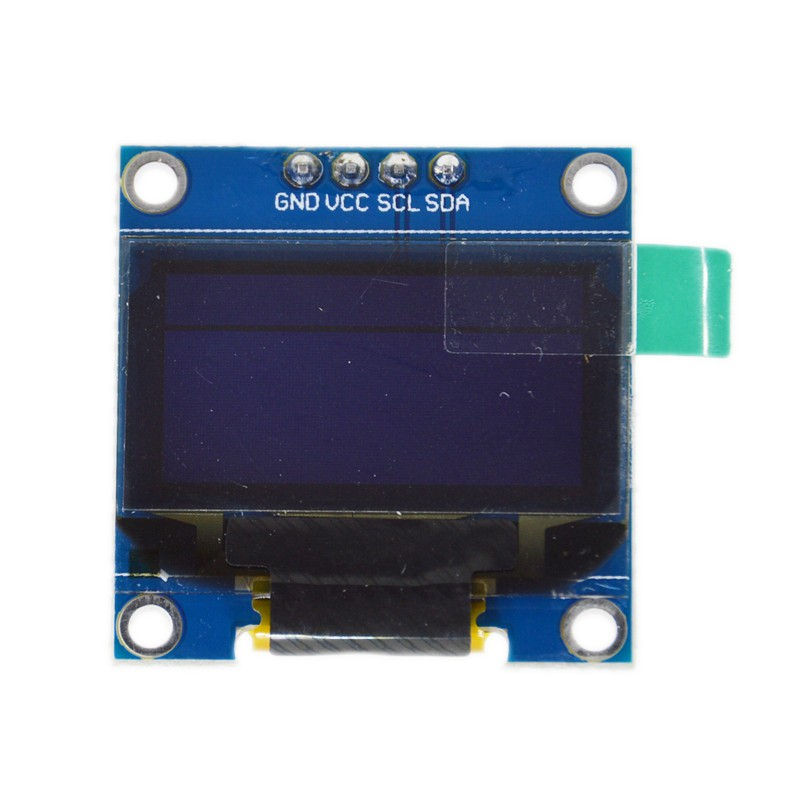
\includegraphics[scale=0.3]{./imagenes/display.jpg}
    \caption{Display OLED SSD1306.}
    \label{F:display}
\end{figure}

\subsection{Aislador I2C capacitivo.}
El dispositivo a utilizar es un ISO1540 \cite{ISO1540} el cual cuenta con buffers de entrada y salida que están separados por tecnología de aislamiento capacitivo de Texas Instruments que utiliza una barrera de dióxido de silicio (SiO2). Cuando se utilizan con fuentes de alimentación aisladas, estos dispositivos bloquean voltajes altos, aíslan tierras y evitan corrientes de ruido que puedan ingresar a la tierra local e interferir o dañar circuitos sensibles. Esta tecnología de aislamiento ofrece ventajas en función, rendimiento, tamaño y consumo de energía en comparación con los optoacopladores. \par 
De este modo tendremos la aislación galvánica para separar apropiadamente la parte de potencia de la de control.
\begin{figure}[H]
    \centering
    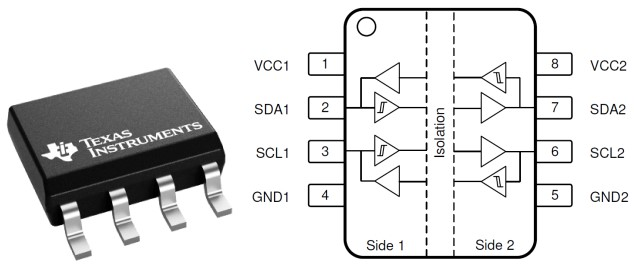
\includegraphics[scale=0.5]{./imagenes/optoi2c.jpg}
    \caption{Aislador capacitivo I2C ISO1540.}
    \label{F:optoi2c}
\end{figure}

\subsection{Convertidor analógico digital. ADC.}
El ADS1115 es un componente crucial en la transición de una fuente de alimentación de corriente continua de analógica a digital. Este dispositivo ofrece una impresionante precisión de 16 bits, junto con una velocidad de muestreo de hasta 860 muestras por segundo a través del protocolo de comunicación I2C. Configurable para operar con cuatro canales de entrada de un solo extremo o dos canales diferenciales, el ADS1115 se destaca por su versatilidad en la medición de señales analógicas en entornos digitales. \par 
Equipado con un conversor delta-sigma de 16 bits, un comparador programable con salida directa al pin de alerta, y una ganancia ajustable que permite la lectura de hasta 256mV en escala completa, este dispositivo garantiza una captura precisa de los datos analógicos. Su interfaz de comunicación I2C facilita la lectura de datos digitales, mientras que su dirección predeterminada de 0x48 y la disponibilidad de bibliotecas para plataformas como Arduino lo convierten en una opción conveniente y de fácil integración en proyectos electrónicos.
\begin{figure}[H]
    \centering
    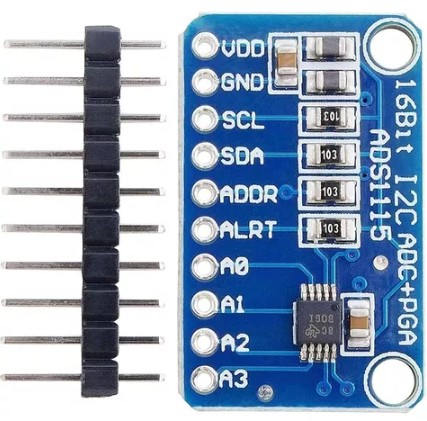
\includegraphics[scale=0.3]{./imagenes/ads1115.jpg}
    \caption{Convertidor AD ADS1115.}
    \label{F:ADC}
\end{figure}

\subsection{Convertidor digital analógico. DAC.}
El MCP4725 es un convertidor digital a analógico (DAC) que permite la conversión precisa de señales digitales en señales analógicas, lo cual es fundamental en aplicaciones donde se requiere una salida de voltaje analógico controlada digitalmente. Este dispositivo ofrece una resolución de 12 bits, proporcionando 4096 niveles de salida posibles y asegurando una alta precisión en la conversión de datos digitales.

Una característica destacada del MCP4725 es su interfaz de comunicación I2C, que permite una fácil integración con microcontroladores y otros dispositivos digitales. Además, incluye una memoria EEPROM interna que puede almacenar la configuración de salida, garantizando que el dispositivo mantenga su valor de salida incluso después de un reinicio.

El MCP4725 es particularmente útil en sistemas embebidos y de control, donde se necesita una conversión precisa y confiable de datos digitales a señales analógicas. Su pequeño tamaño y bajo consumo de energía lo hacen ideal para aplicaciones portátiles y de baja potencia.

\begin{figure}[H]
    \centering
    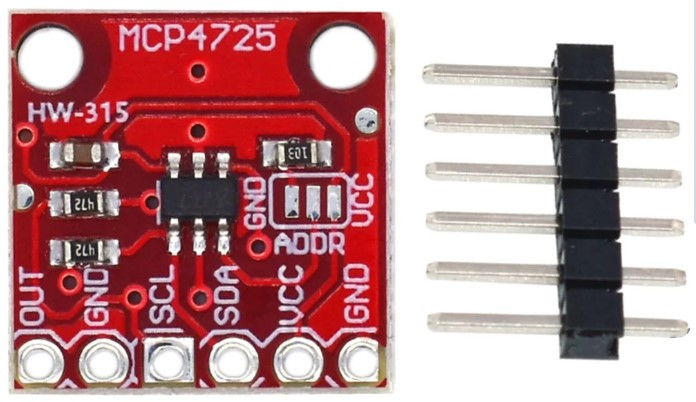
\includegraphics[scale=0.3]{./imagenes/mcp4725.jpg}
    \caption{Convertidor digital analógico MCP4725.}
    \label{F:DAC}
\end{figure}

\section{Modos de operación de la fuente.}
El sistema de control de la fuente de alimentación implementa varios modos de funcionamiento para adaptarse a diversas necesidades de aplicación. A continuación, se describen los principales modos de operación: \par 
\subsection{Modo Tensión}
En este modo, la fuente de alimentación establece inicialmente el valor máximo de tensión deseado. Posteriormente, limita la corriente máxima de umbral que la carga podrá obtener. Este modo es especialmente útil cuando se requiere controlar la tensión suministrada a la carga de manera precisa y garantizar la seguridad del sistema al limitar la corriente máxima.\par 
\subsection{Modo Corriente}
En el modo de corriente, la fuente de alimentación establece y controla la corriente suministrada a la carga. Este modo es útil en situaciones donde es crítico mantener la corriente dentro de ciertos límites para proteger los componentes de la carga y garantizar su correcto funcionamiento.\par 
\subsection{Modo Rampa}
El modo de rampa tiene como objetivo generar un aumento gradual y lineal de la tensión suministrada a la carga durante un período de tiempo determinado. Los parámetros configurables en este modo incluyen la tensión final deseada y el tiempo en el cual se alcanzará esta tensión desde un valor inicial de 0V. Este modo es útil en aplicaciones donde se requiere un inicio suave del sistema para evitar sobrecargas o picos de corriente al arrancar la carga.\par 
